% No preâmbulo: \usepackage{amsmath,amssymb,array,graphicx,placeins}
\section{Fundamentação Teórica}
\label{sec:fun}

Nesta seção são apresentados conceitos sobre criptografia pós-quântica, retomada de sessões, restauração de estado e deduplicação de leituras em redes IoT.

\subsection{Criptografia Pós-Quântica e Sessões Seguras}

A criptografia pós-quântica utiliza algoritmos executados em computadores clássicos, projetados para resistir também a adversários com capacidade computacional quântica \cite{liu2024postquantum}. Esses algoritmos podem atuar no estabelecimento de segredos compartilhados e na autenticação dos participantes da comunicação.

Um mecanismo de encapsulamento de chaves (KEM) permite estabelecer um segredo compartilhado. A partir da chave pública do destinatário, o emissor produz um segredo e uma mensagem de encapsulamento; o destinatário recupera esse segredo com sua chave secreta. Kyber exemplifica uma construção baseada em reticulados \cite{bos2018kyber}. A autenticação exige mecanismos adicionais, como assinaturas digitais, que vinculam mensagens à identidade esperada. Dilithium é um exemplo de assinatura baseada em reticulados \cite{ducas2018dilithium}.

Uma troca híbrida combina contribuições clássicas e pós-quânticas no estabelecimento do segredo. A autenticação pode utilizar assinaturas clássicas ou pós-quânticas, independentemente dessa combinação. Assim, a comparação entre configurações deve identificar tanto a troca de chaves quanto a autenticação empregada, pois ambas influenciam a segurança e o volume de comunicação.

\subsubsection{Estabelecimento Completo e Retomada}

No estabelecimento completo com certificados, os participantes verificam as identidades exigidas pela configuração de confiança e estabelecem as chaves da conexão. Na autenticação mútua, cliente e servidor apresentam suas credenciais. A retomada utiliza um segredo compartilhado de uma sessão previamente autenticada, denominado PSK, reduzindo a repetição de certificados e de operações de autenticação \cite{hebrok2023tickets}.

No TLS 1.3, a retomada pode incorporar uma troca assimétrica efêmera, acrescentando uma contribuição nova à derivação das chaves. A Tabela~\ref{tab:modos_sessao} apresenta essas modalidades. A sessão salva fornece informações para negociar outra conexão, cujas chaves de tráfego são derivadas pelo protocolo.

\begin{table}[!htb]
\centering
\small
\begin{tabular}{|>{\raggedright\arraybackslash}p{0.18\linewidth}|>{\raggedright\arraybackslash}p{0.24\linewidth}|>{\raggedright\arraybackslash}p{0.18\linewidth}|>{\raggedright\arraybackslash}p{0.24\linewidth}|}
\hline
\textbf{Modo} & \textbf{Autenticação} & \textbf{Contribuição nova} & \textbf{Estado requerido} \\
\hline
Completo & Certificados e identidades & Assimétrica & Credenciais e configuração de confiança \\
\hline
Retomada PSK & Segredo anterior & Sem troca assimétrica & Contexto válido \\
\hline
Retomada PSK e DH & Segredo anterior & DH efêmero & Contexto válido e entropia nova \\
\hline
Retomada PSK híbrida & Segredo anterior & DH e KEM efêmeros & Contexto válido e entropia nova \\
\hline
\end{tabular}
\caption{Modalidades de estabelecimento de sessão. DH indica uma troca Diffie--Hellman.}
\label{tab:modos_sessao}
\end{table}

O cliente apresenta um ticket de retomada, cuja aceitação depende de sua validade e das informações disponíveis no servidor. O ticket pode referenciar um registro mantido pelo servidor ou transportar o estado protegido por uma chave. No primeiro caso, o registro precisa permanecer disponível; no segundo, o servidor precisa conservar a chave para recuperar esse estado \cite{hebrok2023tickets}. Portanto, um reinício não implica necessariamente perder a possibilidade de retomada.

Quando a retomada é recusada, a conexão pode prosseguir com autenticação completa, procedimento denominado fallback. Essa negociação pode ocorrer na mesma conexão TLS. Nesse caso, o custo inclui a oferta recusada e a autenticação completa, podendo superar o de iniciar diretamente pelo modo completo. O tamanho da cadeia de certificados e o formato dos tickets também influenciam essa comparação.

A Equação~\ref{eq:custo_recuperacao} representa o custo de recuperação até a confirmação de uma leitura, considerando \(n\) tentativas. \(B_{\mathrm{est},k}\) reúne os bytes de estabelecimento e tickets da tentativa \(k\), incluindo a oferta recusada quando houver. \(B_{\mathrm{app}}\) inclui leituras e confirmações de todas as tentativas; \(B_{\mathrm{extra}}\) reúne os demais bytes contabilizados, como cabeçalhos, retransmissões e encerramentos, sem repetir os anteriores.
\begin{equation}
B_{\mathrm{rec}}=\sum_{k=1}^{n}B_{\mathrm{est},k}+B_{\mathrm{app}}+B_{\mathrm{extra}}.
\label{eq:custo_recuperacao}
\end{equation}

A comparação deve manter o mesmo nível de medição, como registros TLS ou bytes IPv4. O custo de um handshake isolado difere do custo acumulado até a confirmação. Da mesma forma, o tempo de recuperação pode incluir reinícios, novas conexões e reenvios, além do tempo de comunicação.

Chaves diferentes entre conexões não garantem, por si só, sigilo futuro, que busca proteger sessões anteriores diante da exposição posterior de segredos de longo prazo. Essa propriedade depende das contribuições utilizadas e do apagamento dos segredos efêmeros. Construções simétricas com evolução de chaves também investigam sigilo futuro e retomada em IoT \cite{avoine2019iotfriendly}, sob condições diferentes das de um PSK estático conservado.

\subsubsection{Reinícios e Restauração de Estado}

Um reinício elimina dados temporários da memória e recupera informações salvas no armazenamento. Um checkpoint é uma cópia desse estado; restaurar uma versão antiga, procedimento denominado rollback, pode recuperar chaves e contadores já utilizados. Restaurar diretamente uma chave de tráfego difere de apresentar uma sessão salva para uma nova negociação TLS. A perda de um pacote também é um evento distinto, que o transporte pode recuperar sem criar outra sessão.

No AES-GCM, operações distintas de cifragem devem utilizar combinações diferentes de chave e nonce \cite{mcgrew2004gcm}. Na Equação~\ref{eq:unicidade_nonce}, \(K_e\) é a chave de tráfego em uma direção da sessão \(e\), e \(N_{e,i}\) é o nonce da operação \(i\). O requisito abrange operações após reinícios; a retransmissão do mesmo registro já cifrado não constitui outra cifragem.
\begin{equation}
(e,i)\neq(e',j)\ \Longrightarrow\ (K_e,N_{e,i})\neq(K_{e'},N_{e',j}).
\label{eq:unicidade_nonce}
\end{equation}

Restaurar a mesma chave e um contador antigo pode repetir o fluxo de cifragem. A Equação~\ref{eq:reuso_gcm} relaciona segmentos correspondentes de mesmo tamanho dos textos claros \(P_1,P_2\) e cifrados \(C_1,C_2\), excluindo as tags. Conhecer um texto permite recuperar o outro nesse segmento. A reutilização também pode comprometer a autenticidade do GCM \cite{bock2016nonce}.
\begin{equation}
C_1\oplus C_2=P_1\oplus P_2,\qquad
P_2=P_1\oplus C_1\oplus C_2.
\label{eq:reuso_gcm}
\end{equation}

Rejeitar a mensagem no receptor não elimina a informação exposta no tráfego. Autenticar o checkpoint permite detectar adulteração, mas uma cópia antiga e autêntica pode passar nessa verificação. Evitar seu reaproveitamento exige também verificar a atualidade do estado. O estabelecimento de chaves novas depende da autenticação e da disponibilidade de entropia nova.

\subsection{Persistência e Deduplicação de Leituras}

Contadores podem construir nonces distintos sob uma mesma chave. Seu avanço pode ser salvo antes de cada uso ou antecipadamente para um grupo de valores, denominado bloco. Na Equação~\ref{eq:reserva_blocos}, \(a\) é a primeira posição livre, \(b\) é a quantidade reservada e \(q_{\mathrm{salvo}}\) é o limite mantido no armazenamento. A gravação de \(a+b\) deve terminar antes do uso do intervalo.
\begin{equation}
\mathcal{I}_{\mathrm{uso}}=[a,a+b),\qquad q_{\mathrm{salvo}}\leftarrow a+b.
\label{eq:reserva_blocos}
\end{equation}

A Figura~\ref{fig:reserva_estado} apresenta esse procedimento. Após reiniciar, o sensor lê o limite salvo e reserva outro bloco, descartando os valores restantes do anterior. A reserva reduz a frequência de gravação, mas pode deixar posições sem uso. Sua proteção depende de preservar o registro atualizado; restaurar uma cópia antiga pode permitir repetir valores.

\begin{figure}[!htb]
\centering
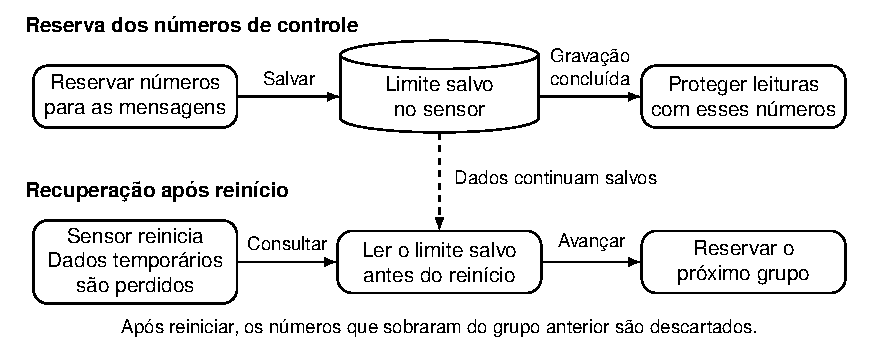
\includegraphics[width=\linewidth]{figuras/figura_1_reserva_contadores.pdf}
\caption{Reserva de números de controle. O limite é salvo antes do uso; após reinício, os valores restantes do bloco anterior são descartados.}
\label{fig:reserva_estado}
\end{figure}

Na aplicação, uma confirmação perdida pode levar ao reenvio de uma leitura já processada. Conservar a identificação da solicitação e seu resultado permite reconhecer novas tentativas e responder sem repetir o efeito \cite{lee2015rifl}. A Figura~\ref{fig:deduplicacao_estado} mostra o gateway consultando o banco após receber novamente o mesmo código de leitura.

\begin{figure}[!htb]
\centering
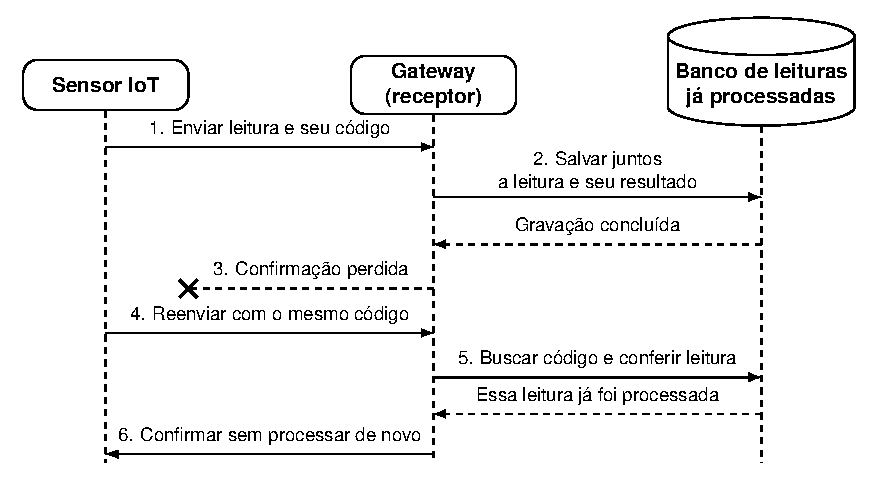
\includegraphics[width=\linewidth]{figuras/figura_2_deduplicacao_leituras.pdf}
\caption{Reconhecimento de uma leitura repetida após perda da confirmação. O gateway consulta o registro salvo e confirma sem repetir o processamento.}
\label{fig:deduplicacao_estado}
\end{figure}

Representamos a leitura por \(r=(d,u,m)\), em que \(d\) identifica o dispositivo, \(u\) identifica a leitura e \(m\) é seu conteúdo. O banco \(L\) associa \((d,u)\) ao resumo criptográfico \(H(m)\). A Equação~\ref{eq:decisao_leitura} distingue leitura nova, repetição com conteúdo correspondente e conflito de conteúdo. A comparação pressupõe resistência a colisões da função de resumo.
\begin{equation}
D(r)=\begin{cases}
\mathrm{nova}, & (d,u)\notin L,\\
\mathrm{repetida}, & (d,u)\in L\ \land\ L[d,u]=H(m),\\
\mathrm{conflito}, & (d,u)\in L\ \land\ L[d,u]\neq H(m).
\end{cases}
\label{eq:decisao_leitura}
\end{equation}

O identificador \(u\) permanece igual nos reenvios e deve distinguir leituras diferentes do mesmo dispositivo, independentemente da chave utilizada para protegê-las. O sensor precisa conservar a leitura pendente e seu identificador até receber a confirmação. No gateway, o registro da leitura, seu resultado e o efeito no banco devem ser salvos atomicamente, isto é, todos são gravados ou nenhum deles é. A gravação deve terminar antes da confirmação e permanecer disponível após reinícios \cite{lee2015rifl}.

Restaurar uma versão antiga do banco pode apagar os registros necessários à deduplicação. Esse histórico pode permanecer disponível após a perda do contexto TLS, pois os dois estados podem ser armazenados separadamente. A proteção descrita abrange os efeitos registrados na mesma operação do banco; atuadores externos exigem coordenação adicional.

\FloatBarrier
